%----------------------------------------------------------------------------------------
%	CHAPTER 3
%----------------------------------------------------------------------------------------

\chapterimage{pano-tv1.png} % Chapter heading image
\acresetall
\chapter{ARCHITECTURE DE L'INTERNET}

\section{Les protocoles}
  
    \vspace{1em}

  \begin{wrapfigure}{r}{8.5cm}
\centerline{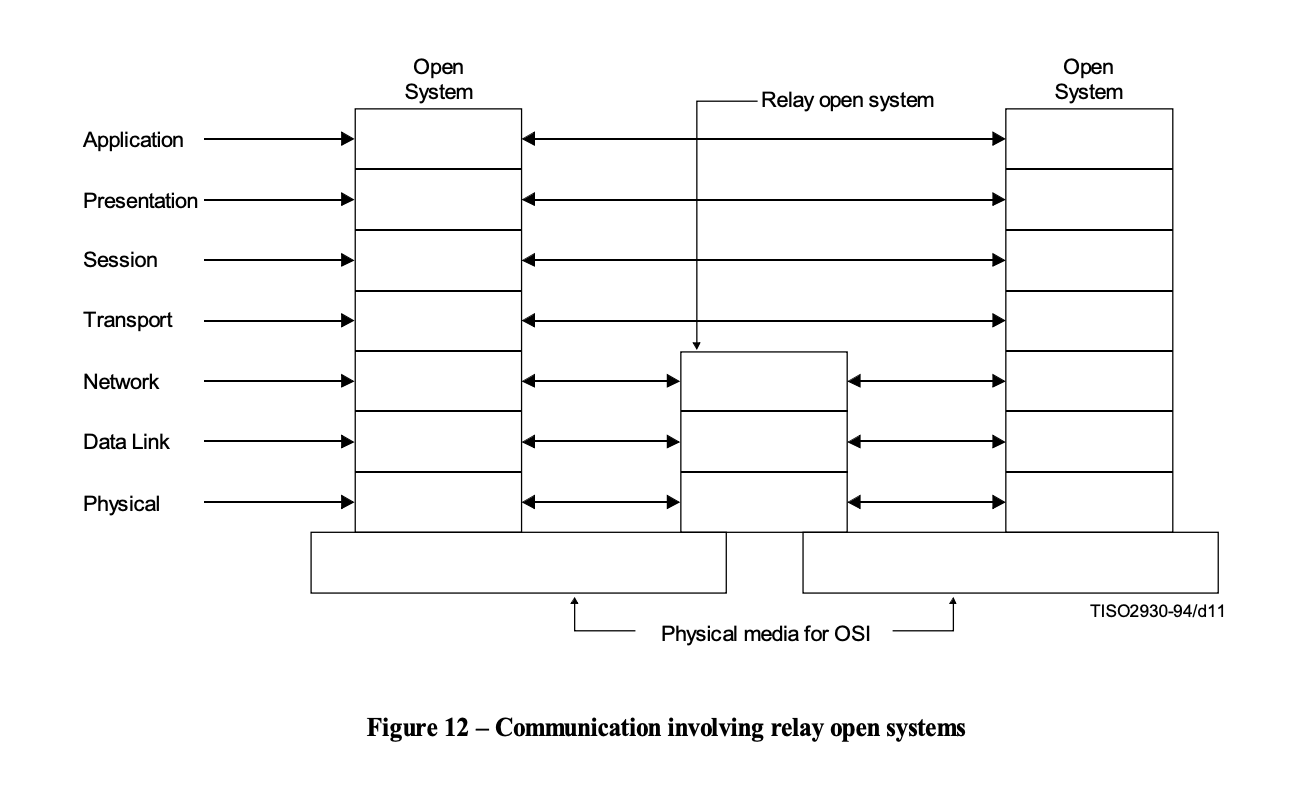
\includegraphics[width=.6\columnwidth]{Pictures/OSI.png}}
\caption{Extrait du standard ITU-T Rec. X.200 (1994 E)}
\end{wrapfigure}

Vous connaissez sûrement le principe d'empilement protocolaire dans les réseaux. Chaque protocole fournit un service et se base sur celui de la couche inférieure pour le réaliser. Le modèle d'origine définit sept couches pour transporter les données d'une application, n'importe où dans le monde.
  Les protocoles réseaux sont empilés les uns sur les autres, ceux du dessus utilisent les services offerts par ceux d’en dessous pour acheminer la donnée. Cela a donné lieu au modèle de référence de l’\ac{ISO} qui structure les réseaux depuis les années 1970. En théorie, il y a 7 \Index{couches}, mais l'internet a fait évoluer ce modèle et les numéros des couches, associés à des fonctionnalités, sont restés ; ce qui peut conduire à une numérotation étrange.
  
 \begin{figure}[tbp]
\centerline{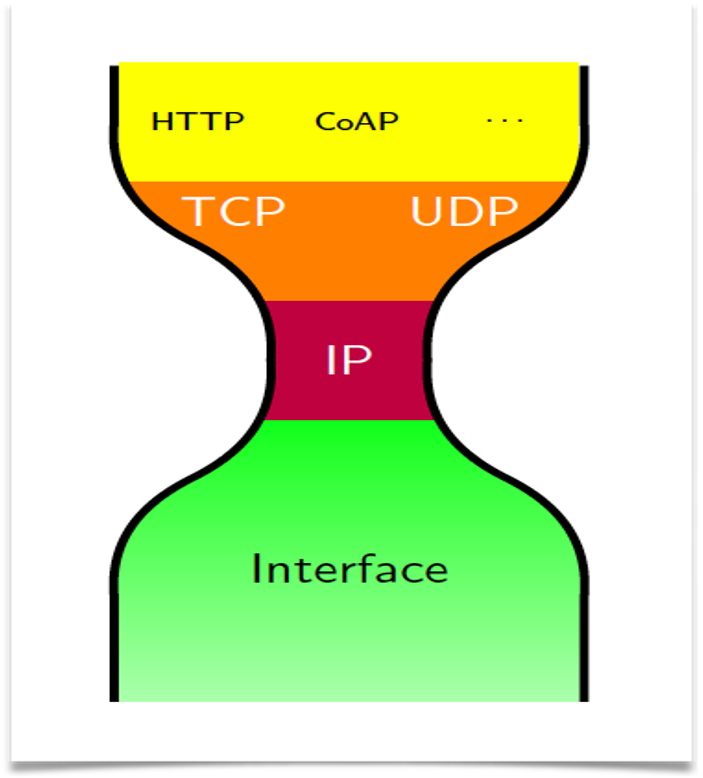
\includegraphics[width=.5\columnwidth]{Pictures/hourglass.png}}
\caption{Empilement protocolaire de l'Internet}
\label{fig-hourglass}
\end{figure}

  \vspace{1em}

\begin{wrapfigure}{r}{3cm}
\Youtube{https://youtu.be/vQ7zMVrqHbA}
\end{wrapfigure}

  L'internet a simplifié cette architecture (cf. figure~\vref{fig-hourglass}). C'est pour ça que l'on retrouve moins de couches et que les numéros ne sont pas contigus. 
  
  
    \vspace{1em}

  Les deux premières couches  en partant du bas, regroupées sous le nom d'Interface, permettent de transmettre les données binaires sur un support physique. La couche 1 s’occupe de cette modulation sur un support physique particulier (fibre optique, paire de cuivre, onde radio). La couche 2 regroupe les mécanismes qui permettent de structurer cette donnée sous forme de bloc de taille finie appelées trames, de définir les méthodes d’accès, c’est-à-dire quand l’équipement peut émettre, et les formats des adresses utilisées pour identifier les équipements. Ethernet ou Wi-Fi sont des exemples de protocoles de niveau 2 (qui intègrent leur niveau 1).

\begin{itemize}
\item l’\ac{IEEE} qui propose des standards comme Ethernet pour les réseaux filaires ou Bluetooth et Wifi pour les réseaux radio,
\item le \ac{3GPP}  qui opère au même niveau et définit les protocoles pour la téléphonie cellulaire (4G),
\item \ldots
\end{itemize}

  
    \vspace{1em}

  
  
  Au-dessus, on a le protocole \ac{IP} standardisé par l'IETF.  Le protocole \ac{IP} s’adapte simplement à tout moyen de communication. \ac{IP} propose ainsi une abstraction des moyens de communication aux couches applicatives, rendant l’accès au réseau et l’adressage universels. Le traitement dans les \Index{routeur}s (équipements chargés d’aiguiller l’information dans le réseau) doit être le plus rapide possible pour traiter un maximum de paquets par seconde. De plus, \ac{IP} ne spécialise pas le réseau pour un service ou un autre ; il ne fait qu’aiguiller les paquets vers la bonne destination. Le réseau Internet est un réseau mondial construit autour de ce protocole permettant potentiellement d'atteindre tous les équipements qui y sont connectés. 
  
  
  Les experts de l'internet aiment cette représentation en \Index{sablier} où \ac{IP} apparaît en position centrale mais est plus petit comparé aux autres protocoles. Par conception, \ac{IP} est très simple ; à la fois pour être portés facilement sur de nombreux niveaux 2 et être facilement utilisable par les couches hautes, mais également pour traiter les données très rapidement dans les nœuds d'interconnexion. 
  
  \ac{IP} est mis en oeuvre partout sur Internet aussi bien dans les équipements en extrémité du réseau que dans les routeurs chargés d'envoyer les données vers la bonne destination.
  
  
    \vspace{1em}

  Au-dessus on trouve deux protocoles qui ne sont mis en oeuvre que dans les équipements d'extrémité.  Si le niveau 3 permet de joindre une machine, le niveau 4 va permettre d’identifier l'application qui doit traiter les données. Les "adresses" de ces applications sont des numéros compris entre 1 et 65535 appelés \Index{port}s. Par exemple, les serveurs Web utilisent le port numéro 80 ou le numéro 443. 
  
  
  Le protocole \ac{TCP} va surveiller les données transférées et sera capable de retransmettre des données perdues, ralentir ou accélérer le transfert de données s’il détecte une saturation du réseau. En revanche, sa mise en œuvre est complexe et coûteuse en mémoire. Dans les cas simple, \ac{UDP} est préféré ; il n'apporte pas de traitement supplémentaire \ac{UDP}, c'est un protocole minimal qui se contentent d'aiguiller les données vers la bonne application sans aucun autre contrôle.
  

    \vspace{1em}

  
  Au-dessus, on trouve les applications qu'historiquement on classe dans la couche 7. Les applications sont très nombreuses mais la plus répandue est \ac{HTTP} qui sert à transporter les pages web, mais également elle permet des communications directes entre ordinateurs. 
  
  
    \vspace{1em}


   \begin{figure}[tbp]
\centerline{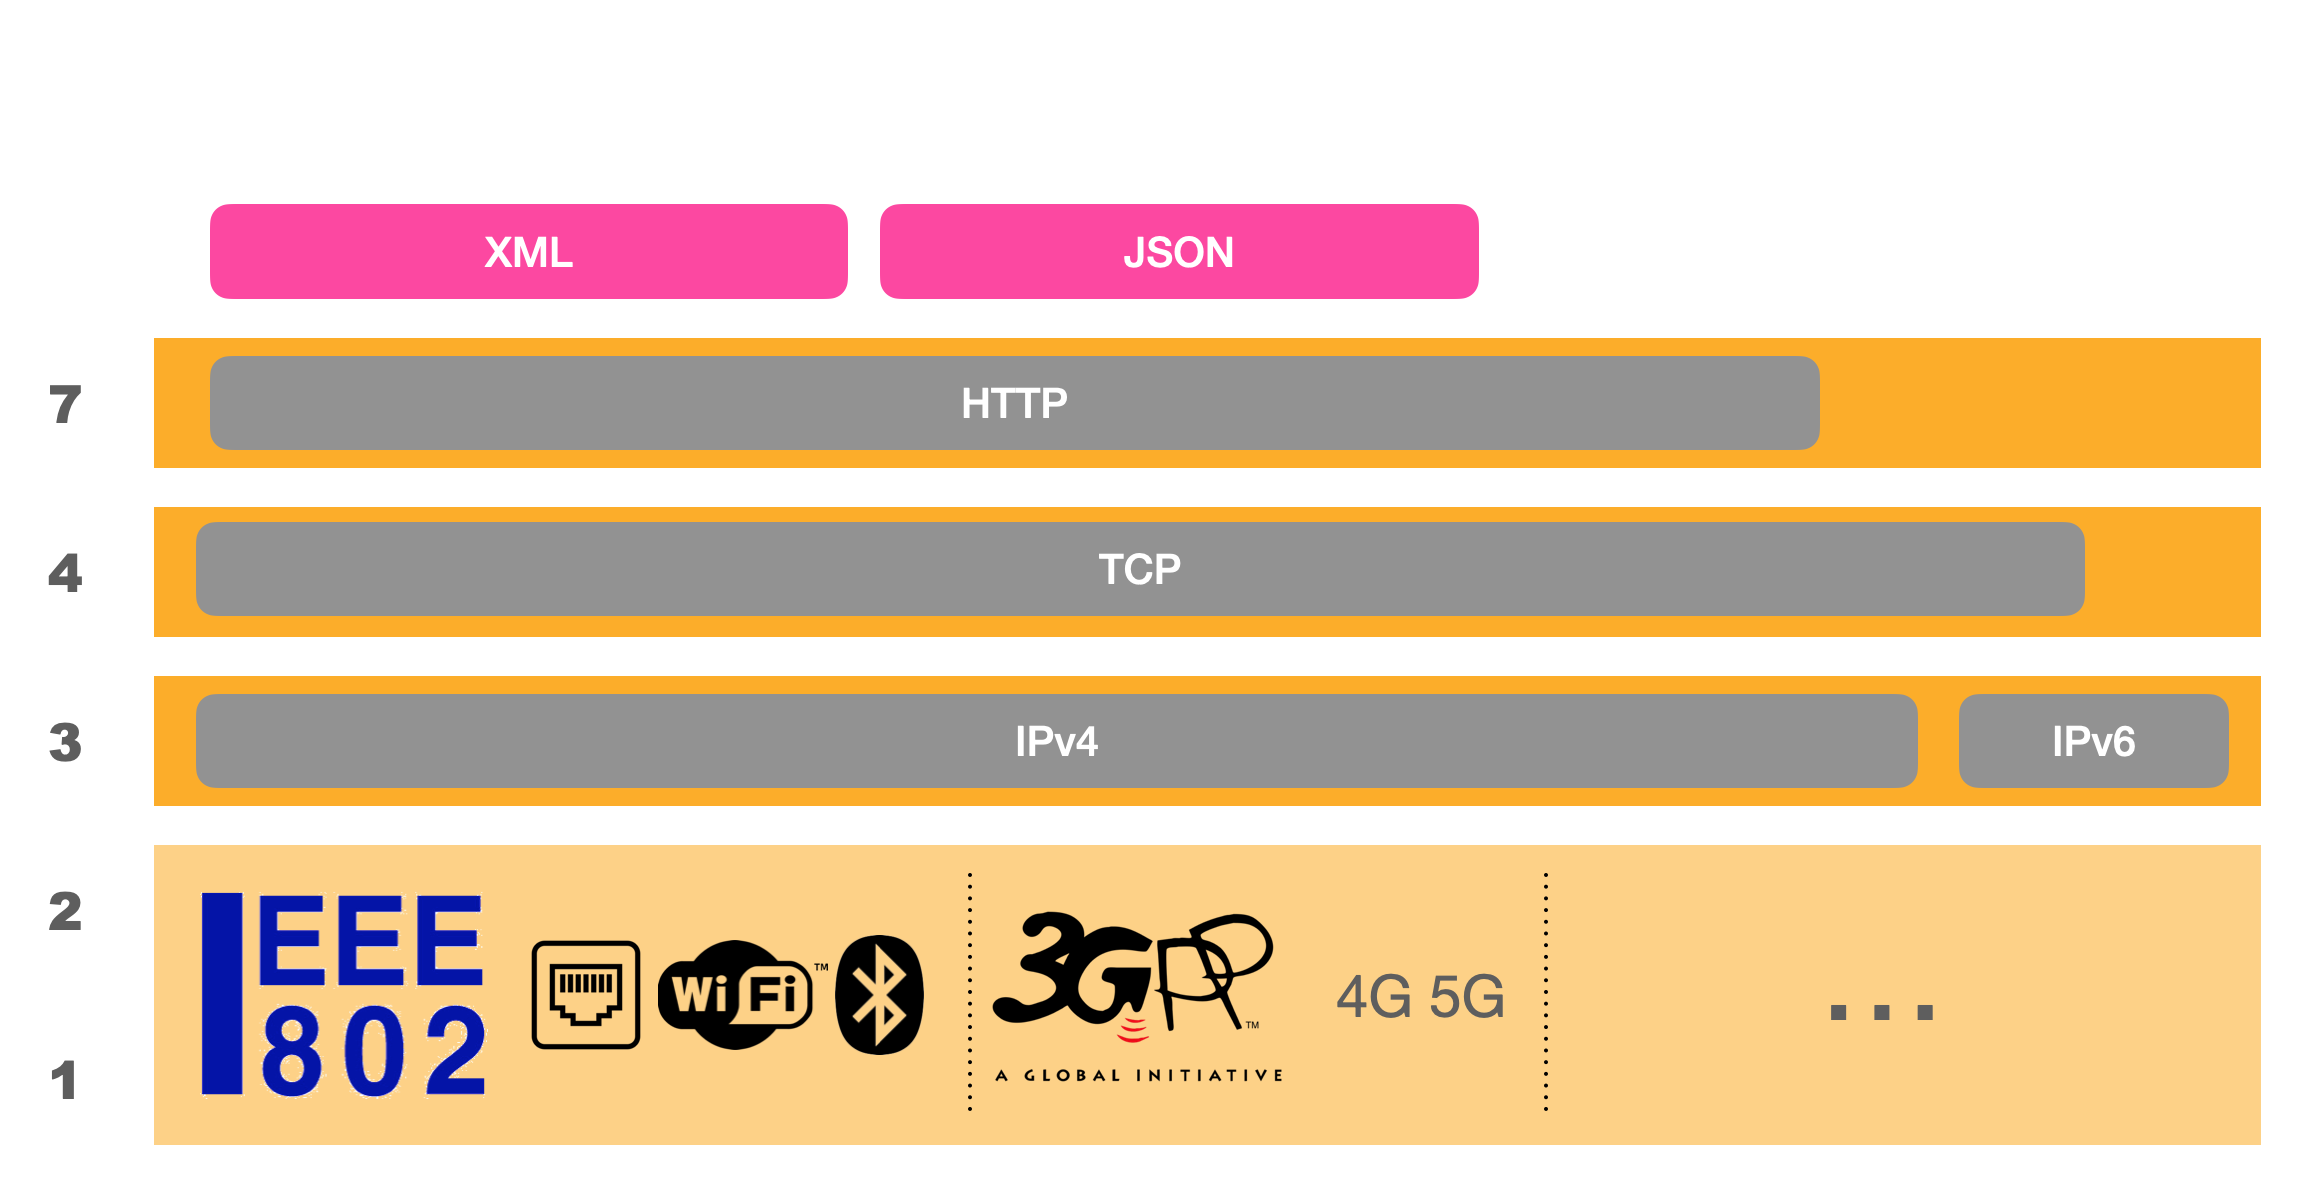
\includegraphics[width=1\columnwidth]{Pictures/fullIPstack.png}}
\caption{Principaux protocoles de l'Internet}
\label{fig-fullstack}
\end{figure}

  Pour le grand public, l’internet désigne surtout la totalité de cet assemblage protocolaire et est souvent confondu avec l’application qui a démocratisé son usage : le Web.  C'est vrai également pour les techniciens, le trafic produit par le Web est largement présent dans l'Internet. Ce schéma, figure~\vref{fig-fullstack} reprend la pile protocolaire majoritairement utilisé dans l'internet. On voit qu'au niveau 3 on a deux versions du protocole \ac{IP} ; la version 4 est la version historiquement déployée et elle a eu tellement de succès qui est de plus en plus difficile d'avoir des adresses \ac{IPv4} pour les machines. Pour permettre au réseau de continuer de fonctionner, une nouvelle version a été développée. \ac{IPv6} rend l'adressage quasi infini avec des adresses sur 128 bits. \ac{IPv6} gagne petit à petit du terrain dans les usages classiques et c'est surtout une brique essentielle pour l'internet des objets. 
  
  Le Web utilise majoritairement le protocole \ac{HTTP}. Et comme \ac{HTTP} repose sur \ac{TCP}, ces deux protocoles sont dominants sur le réseau. 
  
  Finalement ce graphique ajoute une couche supplémentaire, au-dessus de la couche 7, pour indiquer comment les données transportées sont structurées avec des formats comme \ac{XML} ou \ac{JSON} que nous verrons dans la suite.
  
  
  \Question{Pile Protocolaire}
  {Dans la pile protocolaire de l'internet, quels protocoles ont pour fonction d'aiguiller les paquets jusqu'à leur destination (2 réponses) 
  \begin{multicols}{4}
  \begin{itemize}[label=$\square$]
   \item \Wrong{Ethernet}
   \item \Wrong{IEEE}
   \item \Wrong{802.15.5}
   \item \Wrong{Wi-Fi}
   \item \Correct{IPv4}
   \item \Correct{IPv6}
   \item \Wrong{UDP}
   \item \Wrong{TCP}
   \item \Wrong{MQTT} 
   \item \Wrong{HTTP}
   \item \Wrong{CoAP}
   \item \Wrong{XML}
   \item \Wrong{JSON}
  \end{itemize}
  \end{multicols}
  }
  {Le protocole \ac{IP} permet de transporter l'information d'un bout à l'autre du réseau en utilisant les adresses \ac{IP} contenues dans les paquets. Il existe deux versions de ce protocole \ac{IPv4} initialement déployé et \ac{IPv6} qui offre beaucoup plus de capacité d'adressage.}
  
  \section{Les fondements du Web}
  
    \vspace{1em}
\begin{wrapfigure}{r}{3cm}
\Youtube{https://youtu.be/PKKzV-Vy33s}
\end{wrapfigure}

  L'architecture qui a conduit au Web est une formidable source d’inspiration pour le développement de nouveaux services car il est l’un des plus grands succès reposant sur le réseau Internet. Le Web forme de grands systèmes distribués et repose sur plusieurs principes qui le rendent universel et évolutif. La navigation avec un navigateur n’est que la partie visible du trafic ; les principes du web sont également utilisés pour le streaming vidéo, les échanges entre ordinateurs. 
  
  Le Web et ses extensions sont basés sur un modèle client-serveur. Les serveurs possèdent des ressources et les clients peuvent y accéder ou les modifier grâce à un protocole tel que \ac{HTTP}. Le modèle client-serveur est quelque chose de courant dans les réseaux informatiques, mais le Web suit certaines directives de conception connues sous le nom de \ac{REST}.

    \vspace{1em}

Selon Roy Fielding, qui a défini ce modèle~\cite{rest}, \ac{REST} est un ensemble de principes, de propriétés et de contraintes. \ac{REST} utilise le modèle de communication client-serveur et utilise généralement le protocole \ac{HTTP}.

Le principe \ac{REST} permet de concevoir des serveurs évolutifs. Un serveur doit être sans état, ce qui signifie qu’il ne conserve pas d’information après avoir répondu à une demande d’un client. Cela permet de simplifier le traitement dans le serveur qui doit traiter les requêtes d'un grand nombre de clients. 

Cela impose que l’état soit situé du côté du client. Cet état est alimenté à partir des données structurées que le client reçoit du serveur. Ainsi, lorsqu’un client demande une page Web, celle-ci peut contenir d’autres \ac{URI} pour la compléter, par exemple des images, des feuilles de style, des scripts, etc.

Le client doit donc comprendre les données que le serveur lui envoie et donc connaître le format de représentation de la ressource qu'il reçoit pour y retrouver les \ac{URI}. Donc, en plus de la ressource elle-même, le serveur ajoute des informations complémentaires, appelées métadonnées. Elles intègrent entre autres le format du contenu (content format). Il peut s’agir de texte pur, d’une image ou d’un format de texte structuré tel que \ac{HTML} ou \ac{JSON}.
  
      \vspace{1em}

\subsection{Ressources}

    \vspace{1em}

   \begin{wrapfigure}{r}{9cm}
\centerline{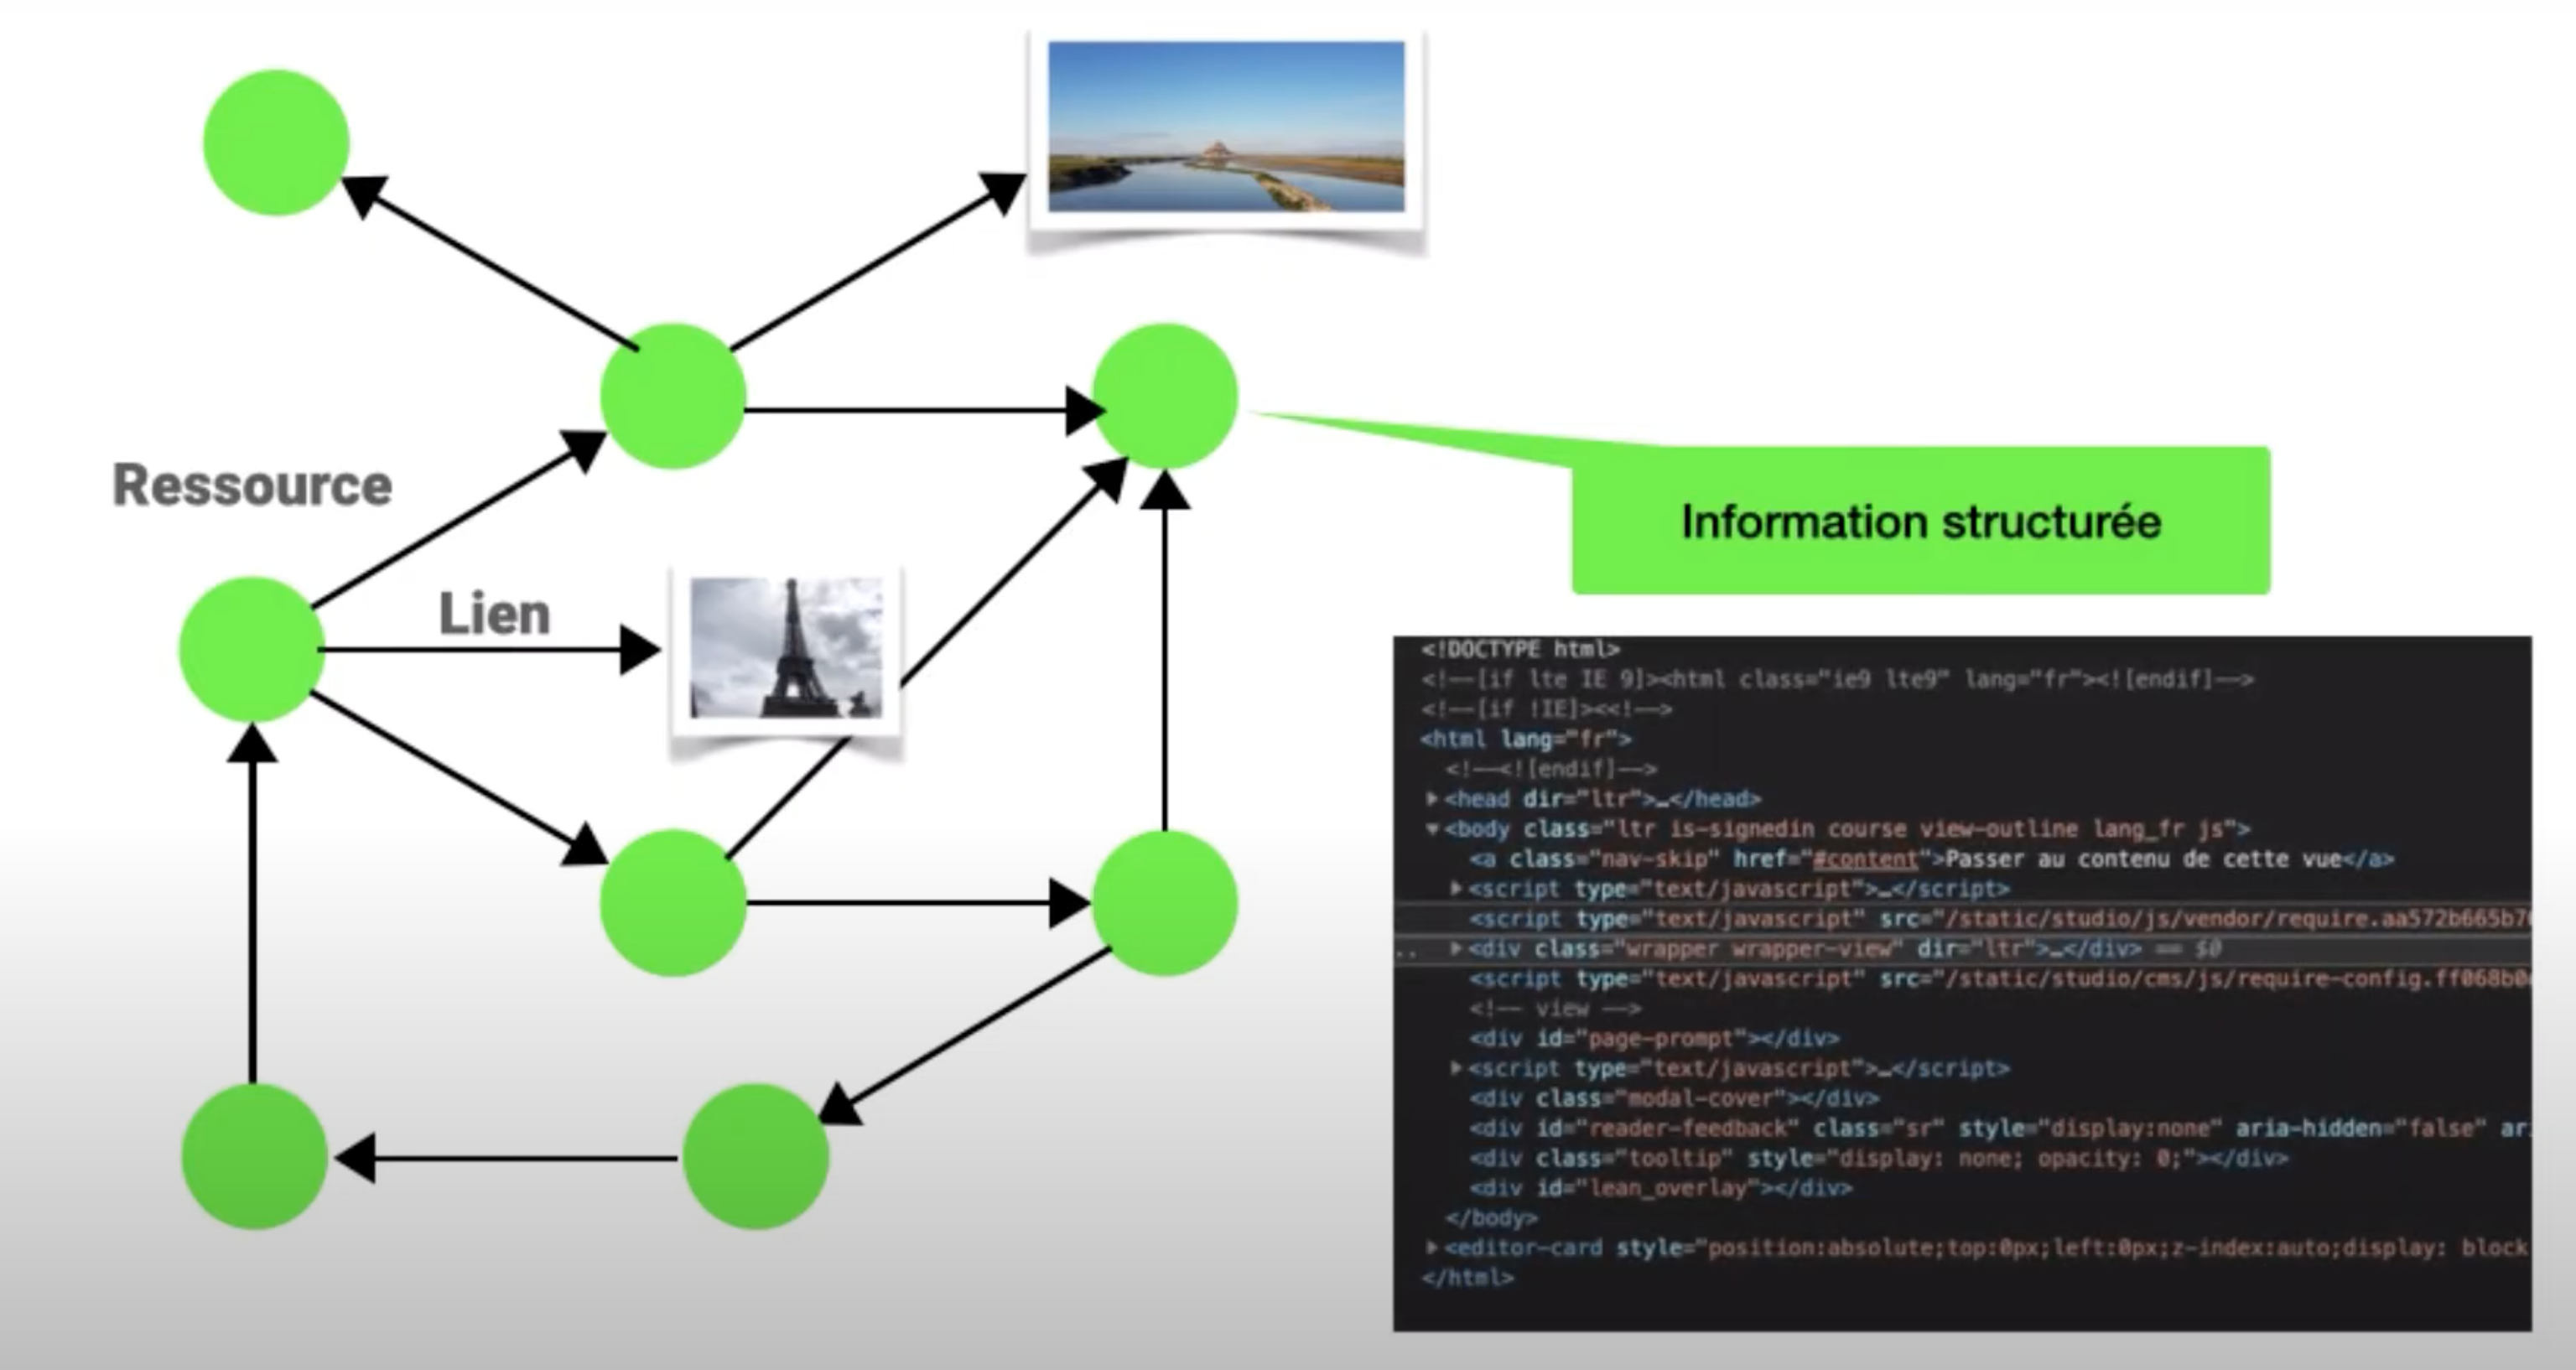
\includegraphics[width=.6\columnwidth]{web.png}}
\end{wrapfigure}
   L'élément de base est la ressource que l'on peut définir comme un bloc de données de taille finie. Les ressources peuvent elles-mêmes contenir des références à d'autres ressources qui à leur tour vont faire référence à d'autres ressources etc. etc. Cela forme un maillage entre ressources qui est comparé à une toile d'araignée (web en anglais). La ressource peut être, par exemple, une image dans ce cas elle ne fera pas référence à autre chose. Pour faire référence à une autre ressource, son contenu doit être structuré et doit donc être défini dans un format où l'on peut facilement comprendre qu'une partie du contenu est une référence a une autre ressource. HTML est un de ces langages qui permet aux pages web de se référencer entre elles par le biais de liens. 
  
      \vspace{1em}

\subsection{identifiants} 

    \vspace{1em}

   
   Chaque ressource du Web est identifiée par une valeur unique appelée \ac{URI}. Si l’URI contient des caractères internationaux, (comme les lettres accentuées, ...)   il est appelé \ac{IRI}.

Les \ac{URI} permettent de désigner une ressource de manière non ambiguë, c'est-à-dire que l'on ne retrouvera pas le même \ac{URI} pour désigner deux ressources différentes.  Par construction, la structure de l’\ac{URI} est hiérarchique, ce qui permet de créer des identificateurs uniques de manière distribuée. Si vous voulez identifier une ressource, vous devez posséder une séquence unique : un numéro de téléphone, un numéro de sécurité sociale, un nom de domaine. En y ajoutant quelque chose d'unique pour nous, cela crée un identifiant globalement unique. 

Par exemple, pour identifier une image, on peut la nommer

\begin{lstlisting}[backgroundcolor = \color{yellow!20}]
image
\end{lstlisting}

\noindent

mais il y a peu de chance que ce nom soit unique, d'autres personnes sur Terre ont sûrement eu la même idée. En revanche, si je la fais précéder de mon numéro de téléphone

\begin{lstlisting}[backgroundcolor = \color{yellow!20}, 
                    basicstyle= \ttfamily]
33667789078image
\end{lstlisting}

\noindent
 sera unique si je ne nomme qu'une seule ressource "image". Un autre utilisateur sur le même principe pourra nommer sa ressource :

\begin{lstlisting}[backgroundcolor = \color{yellow!20}, 
                    basicstyle= \ttfamily]
33667239018image
\end{lstlisting}

\noindent
sans ambiguïté possible. Cependant, comme le numéro de téléphone est unique dans l'espace des numéros de téléphone, d'autres numéros uniques pourraient entrer en conflit dans d'autres espaces de numérotation. 

Pour éviter les conflits, il est intéressant de donner, au début l'espace de numérotation, par exemple :

\begin{lstlisting}[backgroundcolor = \color{yellow!20}, 
                    basicstyle= \ttfamily]
tel:33667789078image
\end{lstlisting}

\noindent
et

\begin{lstlisting}[backgroundcolor = \color{yellow!20}, 
                    basicstyle= \ttfamily]
ss:33667789078image
\end{lstlisting}

\noindent
Les deux identifiants seront uniques, même si le hasard a fait que ce numéro de téléphone et ce numéro de sécurité sociale coïncident.

      \vspace{1em}


Les \ac{URI} formalisent ce principe. Le \rfc{3986} explique comment ils peuvent être construits. Un URI commence par un schéma indiquant l’autorité de nommage, suivi d’une valeur d’autorité puis d’un chemin dans l’espace d’autorité. Des caractères comme les ":" ou les "/" sont utilisés pour améliorer la lisibilité de l'\ac{URI}.



Par exemple~:

\begin{lstlisting}[backgroundcolor = \color{yellow!20}, 
                    basicstyle= \ttfamily]
mailto:mduerst@ifi.unizh.ch
ssh://utilisateur@example.com
ftp://ftp.is.co.za/rfc/rfc1808.txt
\end{lstlisting}

      \vspace{1em}

Ainsi, si je mets une ressource sur un site Web, celui-ci est identifié par un nom de domaine, par exemple \texttt{example.com}. Je suis propriétaire de ce nom. Je peux donc l’utiliser pour identifier de manière unique ma ressource. Si on reprend le principe de construction d’un URI, j’aurai :

\begin{lstlisting}[backgroundcolor = \color{yellow!20}, 
                    basicstyle= \ttfamily]
http://example.com/ma_ressource
\end{lstlisting}

Personne d’autre dans l’univers ne pourra identifier ses ressources avec cette chaîne de caractères puisque \texttt{example.com} m’appartient. Je dispose donc d’un espace de nommage infini qui me permet de désigner l’ensemble infini de ressources sans que personne d’autre ne puisse prendre les mêmes noms. Un \ac{URI} est une construction administrative permettant d’attribuer un identifiant unique global à une ressource spécifique.


  \begin{figure}[tbp]
\centerline{
\includegraphics[width=1\columnwidth]{Pictures/Capture15.png}}
\caption{Structuration d'une URI}
\label{fig-stucURI}
\end{figure}

L’\ac{URI} (cf.figure~\vref{fig-stucURI}) a pour but de facilement nommer une ressource, de pouvoir lier les ressources entre elles pour former cette toile d’araignée mondiale. Le schéma définit à la fois l'espace de nommage de l'autorité et son format. Une adresse \ac{IP} ou un nom de domaine comme autorité est à la fois un moyen d'assurer l'unicité globale, mais également de savoir comment accéder à la ressource. 

      \vspace{1em}

   Par exemple, \Index{spotify} a défini son propre schéma et ensuite il n'a plus besoin d'autorité mais structure le chemin pour référencer une playlist. 
   
   
   
   Tous les livres ont un numéro \ac{ISBN} qui permet d'identifier. Il peut être intégré aussi dans une URI. Il faut voir que ces deux types d'identifiants permettent de référencer un objet unique mais rien qu'en le lisant on ne peut pas accéder à la ressource. On appelle cette sous famille des \ac{URI}, des \ac{URN}. Si en revanche, en lisant l'URI on peut localiser la ressource on a une \ac{URL}.

Un sous-ensemble d’\ac{URI} peut être directement utilisé pour localiser la ressource, c’est-à-dire trouver sur quel serveur se trouve la ressource et comment y accéder. Il s’agit d’une URL bien connue du grand public et utilisée par les navigateurs Web.

Le schéma http est bien pratique car il peut se lire également comme un \ac{URL}. Ce schéma donne~:

\begin{itemize}
\item le protocole à utiliser pour accéder à la ressource (http),
\item l’autorité qui indique l’adresse du serveur (et son port),
\item et enfin, le chemin d’accès de ce que l'on va demander au serveur et qui peut parfois correspondre à une arborescence de fichiers sur un serveur.
\end{itemize}
   
   
       \vspace{1em}

  Mais il faut bien voir que le but initial est de faire un identifiant unique. Le schéma https donne la manière dont sera construit la suite et dans un second temps uniquement sera vu comme le protocole à utiliser pour accéder à la ressource. L'autorité est unique et dans un second temps servira à localiser le serveur. Et finalement le chemin va indiquer comment parvenir à accéder à la ressource sur le serveur. Donc les ressources de notre toile d'araignée mondiale sont présentes sur des serveurs et chaque ressource possède un identifiant unique. Dans un premier temps, le client connaît l'\ac{URI} d'une ressource. Si c'est une \ac{URL}, il peut contacter le serveur. Le serveur lui retourne la ressource. Le client l'analyse et découvre les \ac{URI} qu'il contient. Il peut donc interroger le ou les autres serveurs pour reconstruire localement une partie de la toile nécessaires au traitement que le client veut effectuer.
  
         \vspace{2em}

\Question{Unicité}{Qu'est ce qui est unique dans le monde (6 réponses) ?
\begin{itemize}[label=$\square$]
\item \Wrong{Un prénom.}
\item \Wrong{Un nom de famille.}
\item \Correct{un numéro de sécurité sociale utilisé en France.}
\item \Correct{un numéro de passeport.}
\item \Correct{un numéro de téléphone portable avec son préfixe international.}
\item \Correct{un numéro complet de compte en banque (\ac{IBAN}).}
\item \Wrong{l'adresse IP de ma machine dans mon réseau privé.}
\item \Correct{l'adresse IP d'un serveur fun-mooc (\texttt{51.255.9.16}).}
\item \Correct{le nom de domaine \texttt{plido.net}.}
\item \Wrong{le nom d'une ville.}
\end{itemize}}
{Ni le prénom, ni le nom de famille, ni leur combinaison ne forment des séquences uniques comme le dirait Jean Dupont.
Les numéros de passeport, de sécurité sociale, de téléphone, de compte bancaire sont par construction uniques dans leur espace, mais il pourrait y avoir des recouvrements. C'est pour cela qu'il faut indiquer la source ou l'autorité qui l'a alloué pour garantir l'unicité. Pour le passeport, l’autorité est le pays qui l’a produit. Le numéro de sécurité sociale correspond au numéro d'inscription au  \ac{RNIPP} (cf. \url{https://www.service-public.fr/particuliers/vosdroits/F33078}). Le code du pays pour le numéro de téléphone est attribué par l'UIT puis chaque opérateur a sa zone de numérotation. Pour le compte bancaire, c’est bien sûr la banque ; chaque banque ayant son propre code contenu au début de l'\ac{IBAN}.
L'adresse IP dans un réseau privé n'est pas unique. Le \rfc{1918} définit des plages d'adresses que tout le monde peut utiliser localement. Pour sortir sur Internet, il faut un dispositif spécial, appelé \ac{NAT}, qui va convertir l'adresse privée en une adresse publique qui, elle, est unique dans le monde. Les serveurs doivent être dans cet espace public et ont donc une adresse unique dans le monde.
Les noms de domaines sont uniques dans le monde par construction mais il peuvent être partagés par plusieurs utilisateurs. On peut donc les étendre comme \texttt{machine1.plido.net}, \texttt{machine2.plido.net}... ou, s'il s'agit de la même machine, ajouter un numéro de port après pour indiquer le service : \texttt{www.plido.net:80}, \texttt{www.plido.net:8080}.
Quant au nom d'une ville, il n'est pas unique. Il faut aussi préciser le pays, voire la région.
}
 

  \subsection{Interactions}
  
         \vspace{1em}

  Les interactions entre clients et serveurs sont très simples. Le client va gérer les interactions avec les ressources sur un serveur. Il peut, par exemple, récupérer une ressource grâce à une méthode \Index{GET}. Il peut également écrire les données dans une ressource existante grâce à une méthode \Index{PUT}. 
  
  Le nombre d'interactions est très limité. \ac{HTTP} ou \ac{HTTPS} est un moyen de mettre en oeuvre ces méthodes. 




\ac{HTTP} est un protocole qui peut être utilisé pour mettre en œuvre un serveur Web les principes de \ac{REST} (qualifié en anglais de \Index{RESTfull}). \ac{HTTP} définit différentes méthodes permettant au client d’interagir avec les ressources sur le serveur~:

\begin{itemize}
    \item \Index{GET} est utilisée pour récupérer la représentation d’une ressource (par exemple page Web, valeur de température d’un capteur, etc.). Par exemple, la figure~\vref{fig-GET} donne le format d’en-tête \ac{HTTP} GET pour récupérer une page Web :

 \begin{figure}[tbp]
\centerline{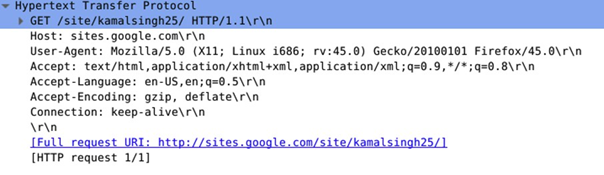
\includegraphics[width=1\columnwidth]{Pictures/GET.png}}
\caption{Contenu d'une requête HTTP GET}
\label{fig-GET}
\end{figure}

\item  \Index{HEAD} est utilisée pour récupérer uniquement les métadonnées présentes dans les en-têtes de réponse sans le corps de réponse ;
\item  \Index{POST} est utilisée pour indiquer au serveur une nouvelle ressource  ;
\item  \Index{PUT} est utilisée pour stocker une ressource à l’endroit identifié par l’\ac{URI} dans la requête. Si la ressource existe déjà, elle sera modifiée ;
\item \Index{PATCH} permet au client de ne modifier qu’une partie de la ressource ;
\item  \Index{DELETE} est utilisée pour supprimer la ressource définie.


\end{itemize}

 \Question{Etat}{Est-ce que le serveur garde un état des précédentes requêtes ?
\begin{itemize}[label=$\circ$]
\item \Wrong{Oui}
\item \Correct{Non}
\end{itemize}}
{Le serveur répond à une requête puis passe à la suivante. Il ne garde pas d'état. En revanche, une requête peut servir à modifier le contenu d'une ressource.}

\Question{Wold Wide Web}{Le World Wide Web est basé sur ce principe des états pour :
\begin{itemize}[label=$\circ$]
\item \Wrong{fonctionner à la fois sur des ordinateurs et des téléphones portables,}
\item \Correct{pouvoir servir un grand nombre de requêtes}

\item \Wrong{chiffrer les communications,}
\end{itemize}}
{Voir le commentaire précédent}

 \Question{Repésentation de l'Information}
  {Quels sont les formats qui permettent de représenter des informations structurées (2 réponses)~: 
  \begin{multicols}{4}
  \begin{itemize}[label=$\square$]
   \item \Wrong{Ethernet}
   \item \Wrong{IEEE}
   \item \Wrong{802.15.5}
   \item \Wrong{Wi-Fi}
   \item \Wrong{IPv4}
   \item \Wrong{IPv6}
   \item \Wrong{UDP}
   \item \Wrong{TCP}
   \item \Wrong{MQTT} 
   \item \Wrong{HTTP}
   \item \Wrong{CoAP}
   \item \Correct{XML}
   \item \Correct{JSON}
  \end{itemize}
  \end{multicols}
  }
  {Il s'agit de XML et JSON qui permettent d'envoyer des données stucturées. Les autres propositions indiquent des protocoles de transport de l'information de niveau 2, 3, 4 et 7.}
  
\Question{Schéma}{Dans l'URI \texttt{https://plido.net/unit/definition.html}, quel est le schéma ?\newline}
{\noindent\texttt{http}~: le Schéma indique comment sera construite l'URI}

\Question{Authorité}{Dans l'URI \texttt{https://plido.net/unit/definition.html}, quel est l'autorité ?\newline}
{\noindent\texttt{plido.net}~: il s'agit de la séquence globalement unique.}


\section {Modèle Publish/Subscribe}

Il existe d’autres formalismes que REST. Un autre formalisme, très populaire, est orienté "diffusion" en utilisant le principe ”publier/abonner” ou ”publish/subscribe”. Comme nous allons le montrer dans la suite, même si les fonctionnalités entre ces deux modes peuvent sembler similaires, la philosophie de conception est très différente : publish/subscribe vise des applications intégrées tandis que REST vise l’interopérabilité globale. 

Le modèle publish/subscribe fait le découplage entre l’expéditeur d’un message et son destinataire. Dans ce paradigme (cf. figure ci-dessous), il existe des ”Publishers” qui produisent des données ou des messages et envoient le message à une entité généralement appelée ”Broker”. En outre, les messages peuvent être classés en ”Topics”, contenus ou types, etc. Ensuite, il existe des abonnés qui souscrivent au broker, par exemple à un topic donné, afin de recevoir les messages qui les intéressent, comme montré dans le schéma.

Le broker peut alors utiliser des filtres pour envoyer uniquement ces messages aux abonnés du topic concerné. Il existe plusieurs protocoles Publish-Subscribe tels que MQTT (Message Queuing Telemetry Transport), AMQP (Advanced Message Queuing Protocol), JMS (Java Messaging Service) ou XMPP (Extensible Messaging Protocol et Présence).

\subsection{MQTT}

MQTT est détaillé dans la suite du cours car il est très populaire pour la communication entre processus, mais également dans l’internet des objets.

Imaginons par exemple que plusieurs capteurs soient installés dans deux bâtiments A et B. Certains capteurs collectent des informations sur la température et d’autres collectent des informations sur l’humidité. Ces capteurs peuvent envoyer les données régulièrement à un broker central.

Les données peuvent être classées en différentes rubriques qui peuvent également être organisées de manière hiérarchique. Par exemple, le topic /sensor signifie "toutes les données de capteurs", \texttt{/sensor/buildingA/} signifie "des données de capteurs uniquement installées dans le bâtiment A". En plus, \texttt{/sensor/buildingA/temperature} pourrait signifier "des données de capteurs de température installés uniquement dans le bâtiment A".

Certains abonnés peuvent s’abonner aux messages en fonction de leur intérêt. Ainsi, un abonné intéressé uniquement par les données d’humidité du bâtiment B peut s’abonner au sujet \texttt{/sensor/buildingB/humidity} et le broker n’enverra que ces données à cet abonné.

\subsection{différence avec REST}

Les principaux avantages du paradigme publish-subscribe par rapport au paradigme client-serveur, tels qu'inclus en REST, sont les suivants :
\begin{itemize}
\item faible couplage entre émetteur et récepteur, le broker sert d'intermédiaire et stocke les informations ;
\item passage à l’échelle. Les données provenant d'une source ne sont émises qu'une fois par la source. Le broker les recopie vers tous les abonnés. Dans un mode client/serveur, les données doivent être émises par le serveur autant que fois que les clients le demandent.
\end{itemize}
L’absence de couplage entre l’expéditeur et le destinataire se fait en termes d’espace, de temps et de synchronisation. Celui qui publie les données a une tâche simplifiée. Il n'a pas à gérer ou connaître ceux qui les consomment, il n'a qu’à les envoyer au broker.

MQTT est très léger et conçu pour les périphériques de faibles puissances. Il a une très petite empreinte logicielle et est optimisé pour fonctionner dans les environnements à faible bande passante. Cela rend MQTT idéal pour les applications IoT. Malgré tout, l’usage de TCP et des très nombreux acquittements peut s’avérer lourds pour les équipements ou les réseaux très contraints. Une version plus légère basée sur UDP existe pour ces cas d’usage, mais elle est peu utilisée.

S'ils se ressemblent, les principes de nommage des topics MQTT et des URI REST sont complètement différents. Par rapport à MQTT, le chemin dans l'URI n'a pas de sémantique. Il a juste vocation à être unique. Il ne peut pas être utilisé pour agréger plusieurs sources d'information. Si deux capteurs publient respectivement sur les topics \texttt{/sensor/buildingA/temperature} et \texttt{/sensor/buildingB/temperature}, un subscriber peut s'abonner au topic \texttt{/sensor/*/temperature} pour recevoir toutes les mesures ; ce qui est impossible avec REST : il faudra autant de requêtes que de capteurs pour récupérer l'ensemble des mesures.

Les URI sont simplement uniques au monde par leur construction alors que les topics du MQTT sont spécifiques à une application. Un topic MQTT peut être interprété différemment par deux applications différentes. Cela ne permet pas une interopérabilité sémantique. Les abonnés doivent être construits avec une connaissance des topics utilisés par les publieurs.
